\documentclass[aspectratio=169]{beamer}

% ---------- ENCODING & FONTS ----------
\usepackage[utf8]{inputenc}
\usepackage[T1]{fontenc}

% ---------- THEME & LOOK ----------
\usetheme{Madrid}
\usecolortheme{seahorse}
\usefonttheme{professionalfonts}
\setbeamertemplate{navigation symbols}{}
\setbeamercovered{transparent}
\setbeamertemplate{itemize items}[circle]
\setbeamertemplate{enumerate items}[default]
\setlength{\parskip}{0.25em}

% ---------- COLORS ----------
% Beamer already loads xcolor, so we just define our colors
\definecolor{accent}{RGB}{0,92,184}
\definecolor{soft}{RGB}{233,244,255}
\definecolor{lightred}{RGB}{245,210,210}
\setbeamercolor{structure}{fg=accent}
\setbeamercolor{title}{fg=white,bg=accent}
\setbeamercolor{frametitle}{fg=accent}
\setbeamercolor{block title}{bg=accent!12,fg=accent}
\setbeamercolor{block body}{bg=soft}

% ---------- PACKAGES ----------
\usepackage{booktabs}
\usepackage{amsmath, amssymb}
\usepackage{array}
\usepackage{multirow}
\usepackage{hyperref}
\hypersetup{colorlinks=true,linkcolor=accent,urlcolor=accent}

% ---------- SAFE TRANSITION FALLBACK ----------
\makeatletter
\@ifundefined{transfade}{\newcommand{\transfade}[1][]{}}{}
\makeatother

% ---------- PLACEHOLDER BOX FOR FIGURES ----------
\newcommand{\placeholderbox}[2][0.82\linewidth]{%
  \begin{center}
    \fbox{\begin{minipage}[c][0.46\textheight][c]{#1}
      \centering \vspace{0.3em}
      \textbf{#2}\\[0.6em]
      \emph{Insert figure/diagram here later.}
    \end{minipage}}
  \end{center}
}

% ---------- TITLE ----------
\title{\textbf{Money, Banks, and the Bank of Canada \vspace{.5cm}\\  }}
\subtitle{ {\large ECON 101 - Macroeconomics}}
%\institute{UNBC}
\author{Muhebullah Karimzada}
\date{Winter 2026}



\begin{document}

% ============================================================
% TITLE
% ============================================================
\begin{frame}[plain]
  \titlepage
\end{frame}

% ============================================================
\begin{frame}{Chapter Outline}
\transfade
\begin{itemize}[<+->]
  \item \textbf{10.1} What Is Money, and Why Do We Need It?
  \item \textbf{10.2} How Is Money Measured in Canada Today?
  \item \textbf{10.3} How Do Banks Create Money?
  \item \textbf{10.5} The Quantity Theory of Money
\end{itemize}
\end{frame}

% ============================================================
\section{10.1 What Is Money, and Why Do We Need It?}
% ============================================================

\begin{frame}{10.1 Learning Objective}
\transfade
\begin{block}{Goal}
Define money and discuss the four functions of money.
\end{block}
\begin{itemize}[<+->]
  \item Understand what economists mean by \alert{money}.
  \item See how money solves problems with barter.
  \item Learn the \textbf{four functions} of money.
  \item Discuss what can and cannot serve as money.
\end{itemize}
\end{frame}

\begin{frame}{What Is Money?}
\transfade
\begin{itemize}[<+->]
  \item \textbf{Money} is \alert{any asset} that people are generally willing to accept:
  \begin{itemize}[<+->]
    \item in exchange for goods and services, or
    \item in payment of debts.
  \end{itemize}
  \item \textbf{Asset:} anything of value owned by a person or a firm.
  \item Money is one of the most important inventions in economic history because:
  \begin{itemize}[<+->]
    \item it makes trade easier,
    \item it allows specialization,
    \item it supports the development of complex economies.
  \end{itemize}
\end{itemize}
\end{frame}

\begin{frame}{Life Without Money: Barter}
\transfade
\begin{itemize}[<+->]
  \item Imagine living before money existed.
  \item All trade would be \textbf{barter}:
  \begin{itemize}[<+->]
    \item trading goods and services directly for goods and services.
  \end{itemize}
  \item Barter requires a \alert{double coincidence of wants}:
  \begin{itemize}[<+->]
    \item you must have what I want,
    \item and I must have what you want,
    \item at the same time and place.
  \end{itemize}
  \item Barter works in small, simple economies, but breaks down as:
  \begin{itemize}[<+->]
    \item the number of goods and services grows,
    \item and people become more specialized.
  \end{itemize}
\end{itemize}
\end{frame}

\begin{frame}{From Barter to Commodity Money}
\transfade
\begin{itemize}[<+->]
  \item To avoid the problems of barter, societies adopted \textbf{commodity money}.
  \item \textbf{Commodity money:}
  \begin{itemize}[<+->]
    \item goods used as money that also have value independent of their use as money.
  \end{itemize}
  \item Examples:
  \begin{itemize}[<+->]
    \item Precious metals such as \alert{gold} and \alert{silver},
    \item Beaver pelts among early settlers and some Indigenous peoples in Canada,
    \item Cigarettes in prisons and prisoner-of-war camps.
  \end{itemize}
  \item Commodity money works as long as people:
  \begin{itemize}[<+->]
    \item value the commodity itself,
    \item and agree to use it in trade.
  \end{itemize}
\end{itemize}
\end{frame}

\begin{frame}{The Four Functions of Money}
\transfade
\begin{itemize}[<+->]
  \item Money fulfills \textbf{four primary functions}:
  \begin{enumerate}[<+->]
    \item \textbf{Medium of exchange}
    \item \textbf{Unit of account}
    \item \textbf{Store of value}
    \item \textbf{Standard of deferred payment}
  \end{enumerate}
\end{itemize}
\end{frame}

\begin{frame}{Function 1: Medium of Exchange}
\transfade
\begin{itemize}[<+->]
  \item Money is a \textbf{medium of exchange} if:
  \begin{itemize}[<+->]
    \item it is acceptable to a wide variety of parties
    \item as payment for goods and services.
  \end{itemize}
  \item Instead of barter:
  \begin{itemize}[<+->]
    \item you sell your labour or goods \(\Rightarrow\) receive money,
    \item then use money to buy what you want.
  \end{itemize}
  \item This greatly reduces the time and effort needed to find trading partners.
\end{itemize}
\end{frame}

\begin{frame}{Function 2: Unit of Account}
\transfade
\begin{itemize}[<+->]
  \item Money is a \textbf{unit of account}:
  \begin{itemize}[<+->]
    \item it provides a standard way of measuring the value of goods and services.
  \end{itemize}
  \item In Canada, prices are quoted in \(\$\) \alert{Canadian dollars}.
  \item Without a unit of account:
  \begin{itemize}[<+->]
    \item every good would have to be priced in terms of every other good.
    \item In a large economy, this would be extremely confusing.
  \end{itemize}
\end{itemize}
\end{frame}

\begin{frame}{Function 3: Store of Value}
\transfade
\begin{itemize}[<+->]
  \item Money is a \textbf{store of value}:
  \begin{itemize}[<+->]
    \item it allows people to transfer purchasing power from today to the future.
  \end{itemize}
  \item Other assets also store value:
  \begin{itemize}[<+->]
    \item stocks, bonds, houses, land, art, etc.
  \end{itemize}
  \item Money is special because it is:
  \begin{itemize}[<+->]
    \item highly \alert{liquid} (easily converted into goods and services),
    \item relatively stable in value in low-inflation economies.
  \end{itemize}
  \item Inflation reduces the effectiveness of money as a store of value.
\end{itemize}
\end{frame}

\begin{frame}{Function 4: Standard of Deferred Payment}
\transfade
\begin{itemize}[<+->]
  \item Money is a \textbf{standard of deferred payment}:
  \begin{itemize}[<+->]
    \item it is widely accepted for settling debts that are paid back in the future.
  \end{itemize}
  \item Loans and credit contracts are typically denominated in money terms.
  \item This works well when:
  \begin{itemize}[<+->]
    \item the value of money is reasonably \alert{predictable} over time.
  \end{itemize}
\end{itemize}
\end{frame}

\begin{frame}{What Can Serve as Money?}
\transfade
\begin{itemize}[<+->]
  \item For an asset to serve as a widely accepted medium of exchange, it should:
  \begin{enumerate}[<+->]
    \item Be \textbf{acceptable} to most people.
    \item Have \textbf{standardized quality} so any two units are alike.
    \item Be \textbf{durable} so it does not wear out quickly.
    \item Be \textbf{valuable relative to its weight}, so it is easy to transport.
    \item Be \textbf{divisible} enough to make both small and large transactions.
  \end{enumerate}
  \item Historical and modern monies (gold coins, bank notes, electronic deposits) satisfy these conditions to different degrees.
\end{itemize}
\end{frame}

\begin{frame}{Commodity Money: Examples}
\transfade
\begin{itemize}[<+->]
  \item \textbf{Commodity money} has value independent of its use as money.
  \item Examples:
  \begin{itemize}[<+->]
    \item Gold and silver coins.
    \item Beaver pelts in early Canadian trade.
    \item Cigarettes used in prisons or war camps.
  \end{itemize}
  \item Advantage:
  \begin{itemize}[<+->]
    \item intrinsic value supports trust in the money.
  \end{itemize}
  \item Disadvantages:
  \begin{itemize}[<+->]
    \item can be costly to store and transport,
    \item supply may be hard to control.
  \end{itemize}
\end{itemize}
\end{frame}

\begin{frame}{Fiat Money (1 of 2)}
\transfade
\begin{itemize}[<+->]
  \item In modern economies, money is typically \textbf{paper currency} issued by a \alert{central bank}.
  \item In Canada, the central bank is the \textbf{Bank of Canada}.
  \item Modern currencies are \textbf{not} convertible into gold or any commodity.
  \item \textbf{Fiat money:}
  \begin{itemize}[<+->]
    \item money, such as paper currency, that is authorized by a central bank or government,
    \item and does not have to be exchanged for a commodity like gold.
  \end{itemize}
\end{itemize}
\end{frame}

\begin{frame}{Fiat Money (2 of 2)}
\transfade
\begin{itemize}[<+->]
  \item Fiat money is more \alert{flexible}:
  \begin{itemize}[<+->]
    \item central banks can adjust the money supply to respond to shocks.
  \end{itemize}
  \item But it also has a potential problem:
  \begin{itemize}[<+->]
    \item it is valuable only as long as households and firms \textbf{have confidence} in it.
  \end{itemize}
  \item If people lose confidence that paper dollars will hold their value:
  \begin{itemize}[<+->]
    \item they will not accept them in exchange,
    \item and fiat money will cease to be useful.
  \end{itemize}
\end{itemize}
\end{frame}

% ============================================================
\section{10.2 How Is Money Measured in Canada Today?}
% ============================================================

\begin{frame}{10.2 Learning Objective}
\transfade
\begin{block}{Goal}
Discuss the definitions of the money supply used in Canada today.
\end{block}
\begin{itemize}[<+->]
  \item Different assets vary in how \textbf{liquid} they are.
  \item The Bank of Canada uses several definitions of the money supply:
  \begin{itemize}[<+->]
    \item from narrow measures (very liquid) to broad measures (include less liquid assets).
  \end{itemize}
\end{itemize}
\end{frame}

\begin{frame}{Figure 10.1 -- Components of the Money Supply (1 of 3)}
\centering
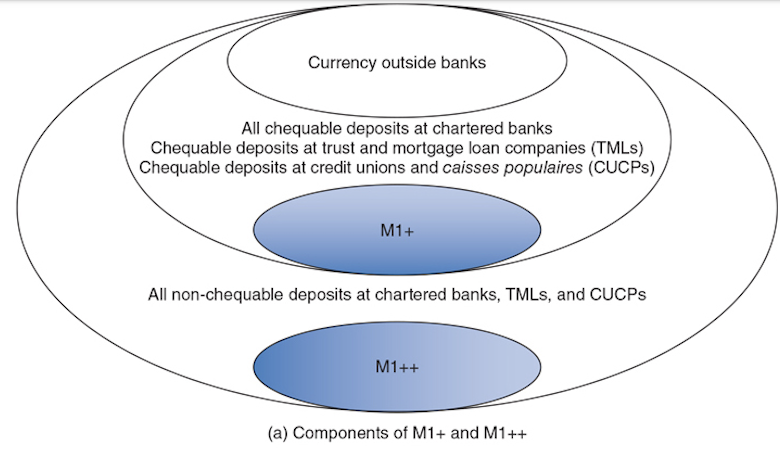
\includegraphics[width=0.8\linewidth]{Fig10-001a}
\end{frame}

\begin{frame}{Figure 10.1 -- Components of the Money Supply (2 of 3) }

\centering
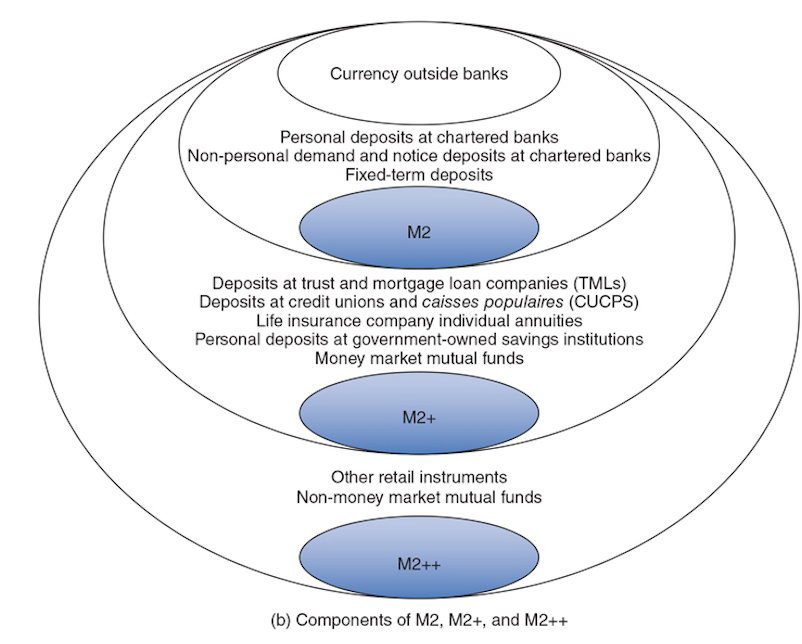
\includegraphics[width=0.6\linewidth]{Fig10-001b}
\end{frame}

\begin{frame}{Figure 10.1 -- Components of the Money Supply (3 of 3) }
\centering
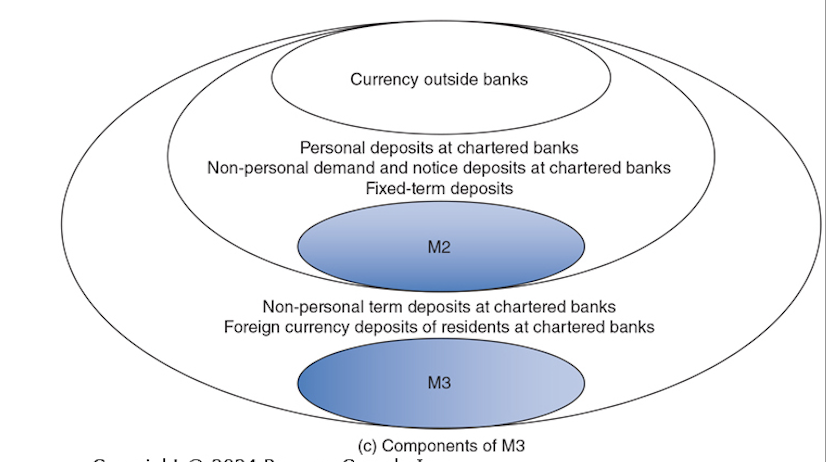
\includegraphics[width=0.8\linewidth]{Fig10-001c}
\end{frame}

\begin{frame}{The Bank of Canada’s Measures of Money}
\transfade
\begin{itemize}[<+->]
  \item The Bank of Canada uses six main measures:
  \begin{itemize}[<+->]
    \item \(\textbf{M1+}, \textbf{M1++}, \textbf{M2}, \textbf{M2+}, \textbf{M2++}, \textbf{M3}\).
  \end{itemize}
  \item \textbf{M1+:} narrowest definition.
  \item \textbf{M2++:} broadest definition.
  \item Each broader measure includes all the assets in the narrower measures, plus some extra, less liquid assets.
\end{itemize}
\end{frame}

\begin{frame}{Definition of M1+ and M1++}
\transfade
\begin{itemize}[<+->]
  \item \textbf{M1+:}
  \begin{itemize}[<+->]
    \item Currency in circulation (bank notes and coins outside banks).
    \item \textbf{Chequable deposits} at:
    \begin{itemize}[<+->]
      \item banks,
      \item trust and mortgage companies,
      \item credit unions and \emph{caisses populaires}.
    \end{itemize}
  \end{itemize}
  \item \textbf{M1++:}
  \begin{itemize}[<+->]
    \item Includes all of M1+,
    \item plus \textbf{non-chequable deposits}.
  \end{itemize}
\end{itemize}
\end{frame}

\begin{frame}{Definition of M2 and M2+}
\transfade
\begin{itemize}[<+->]
  \item \textbf{M2} includes:
  \begin{itemize}[<+->]
    \item Currency,
    \item Personal deposits at banks,
    \item Non-personal demand and notice deposits at banks,
    \item Fixed-term deposits at banks.
  \end{itemize}
  \item \textbf{M2+:} includes M2 plus:
  \begin{itemize}[<+->]
    \item Deposits at trust and mortgage loan companies (TMLs),
    \item Deposits at credit unions and \emph{caisses populaires} (CUCPs),
    \item Life insurance company individual annuities,
    \item Government-owned savings institutions,
    \item Money market mutual funds.
  \end{itemize}
\end{itemize}
\end{frame}

\begin{frame}{Definition of M2++ and M3}
\transfade
\begin{itemize}[<+->]
  \item \textbf{M2++} (broadest measure):
  \begin{itemize}[<+->]
    \item Includes M2+ plus:
    \begin{itemize}[<+->]
      \item Canada Savings Bonds,
      \item Non-money market mutual funds.
    \end{itemize}
  \end{itemize}
  \item \textbf{M3} includes:
  \begin{itemize}[<+->]
    \item M2,
    \item Non-personal term deposits at banks,
    \item Foreign-currency deposits of Canadians at banks.
  \end{itemize}
\end{itemize}
\end{frame}

\begin{frame}{Which Money Supply Measure to Use?}
\transfade
\begin{itemize}[<+->]
  \item Any of the main measures might be relevant, depending on the question.
  \item For most macroeconomic analysis, we focus on money as a \textbf{medium of exchange}.
  \item That suggests concentrating on \textbf{M1+}:
  \begin{itemize}[<+->]
    \item currency in circulation,
    \item chequable deposits.
  \end{itemize}
  \item In our discussion:
  \begin{itemize}[<+->]
    \item we treat both currency and chequing/non-chequing account balances as “money”,
    \item but not the broader set of financial assets.
  \end{itemize}
\end{itemize}
\end{frame}

% ============================================================
\section{10.3 How Do Banks Create Money?}
% ============================================================

\begin{frame}{10.3 Learning Objective}
\transfade
\begin{block}{Goal}
Explain how banks create money.
\end{block}
\begin{itemize}[<+->]
  \item Banks are central to the money creation process.
  \item More money is held in chequing accounts than exists as physical currency.
  \item Banks are profit-making private firms; they:
  \begin{itemize}[<+->]
    \item accept deposits,
    \item make loans,
    \item and thereby \alert{create money}.
  \end{itemize}
\end{itemize}
\end{frame}

\begin{frame}{Figure 10.2 -- Balance Sheet for Royal Bank  }
\centering
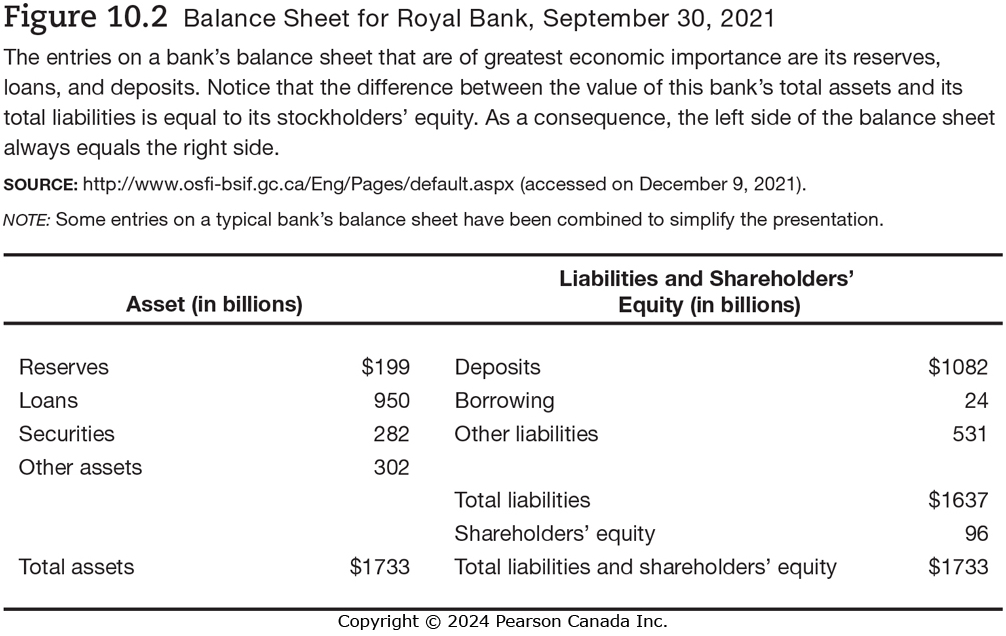
\includegraphics[width=0.9\linewidth]{Fig10-002}
\end{frame}



\begin{frame}{Bank Balance Sheets: Assets and Liabilities}
\transfade
\begin{itemize}[<+->]
  \item On a \textbf{balance sheet}:
  \begin{itemize}[<+->]
    \item Assets are listed on the left,
    \item Liabilities and stockholders' equity (\textbf{net worth}) on the right.
  \end{itemize}
  \item \textbf{Assets} for a bank include:
  \begin{itemize}[<+->]
    \item Reserves (cash in vaults and deposits at the Bank of Canada),
    \item Loans,
    \item Securities and other investments.
  \end{itemize}
  \item \textbf{Liabilities} include:
  \begin{itemize}[<+->]
    \item Deposits (chequing, savings, term deposits),
    \item Borrowings.
  \end{itemize}
  \item The two sides must always sum to the same total.
\end{itemize}
\end{frame}

\begin{frame}{Reserves and Desired Reserve Ratio}
\transfade
\begin{itemize}[<+->]
  \item \textbf{Reserves:}
  \begin{itemize}[<+->]
    \item deposits that a bank keeps as cash in its vault or on deposit with the Bank of Canada.
  \end{itemize}
  \item Banks in Canada are \textbf{not} required to hold a specific level of reserves by law.
  \item They choose to keep a fraction of deposits on hand as reserves:
  \begin{itemize}[<+->]
    \item often around 5\%.
  \end{itemize}
  \item \textbf{Desired reserve ratio} (\(r_{d}\)):
  \begin{itemize}[<+->]
    \item the fraction of deposits banks \emph{want} to keep as reserves.
  \end{itemize}
  \item Banks may adjust \(r_{d}\) depending on:
  \begin{itemize}[<+->]
    \item the state of the economy,
    \item and financial market conditions.
  \end{itemize}
\end{itemize}
\end{frame}

\begin{frame}{T-Accounts: A Simple Tool}
\transfade
\begin{itemize}[<+->]
  \item A \textbf{T-account} is a simplified balance sheet.
  \item It shows only how a transaction \alert{changes} assets and liabilities.
  \item Example: you deposit \$1{,}000 in currency at Bank of Montreal (BMO).
  \item BMO's T-account change:
  \begin{center}
    \begin{tabular}{p{0.4\linewidth} p{0.4\linewidth}}
    \toprule
    \multicolumn{1}{c}{\textbf{Assets}} & \multicolumn{1}{c}{\textbf{Liabilities}} \\
    \midrule
    Reserves \(\,+ \$1{,}000\) & Deposits \(\,+ \$1{,}000\) \\
    \bottomrule
    \end{tabular}
  \end{center}
  \item The currency component of the money supply falls by \$1{,}000, but chequing deposits rise by \$1{,}000, so total money supply is unchanged \textbf{so far}.
\end{itemize}
\end{frame}

\begin{frame}{From Deposits to Loans: Creating New Money}
\transfade
\begin{itemize}[<+->]
  \item BMO holds some of the \$1{,}000 as reserves and lends out the rest.
  \item Suppose it keeps 10\% (\$100) as reserves and lends \$900.
  \item T-account changes for BMO after the loan:
  \begin{center}
    \begin{tabular}{p{0.4\linewidth} p{0.4\linewidth}}
    \toprule
    \multicolumn{1}{c}{\textbf{Assets}} & \multicolumn{1}{c}{\textbf{Liabilities}} \\
    \midrule
    Reserves \(\,+ \$1{,}000\) & Deposits \(\,+ \$1{,}000\) \\
    Loans \(\,+ \$900\) & Deposits \(\,+ \$900\) \\
    \bottomrule
    \end{tabular}
  \end{center}
  \item The \$900 loan is typically deposited at another bank, so:
  \begin{itemize}[<+->]
    \item the banking system now has:
    \begin{itemize}[<+->]
      \item \$1{,}000 in new reserves,
      \item \$1{,}900 in deposits.
    \end{itemize}
  \end{itemize}
\end{itemize}
\end{frame}

\begin{frame}{Multiple Rounds of Money Creation}
\transfade
\begin{itemize}[<+->]
  \item The process continues across banks:
  \begin{itemize}[<+->]
    \item each bank keeps 10\% of new deposits as reserves,
    \item and lends out the remaining 90\%.
  \end{itemize}
  \item First deposit: \$1{,}000 reserves.
  \item First loan: \$900 new deposit in the system.
  \item Second round:
  \begin{itemize}[<+->]
    \item 10\% of \$900 (i.e., \$90) kept as reserves,
    \item \$810 loaned out and deposited.
  \end{itemize}
  \item Third round:
  \begin{itemize}[<+->]
    \item 10\% of \$810 kept as reserves,
    \item \$729 loaned out, etc.
  \end{itemize}
\end{itemize}
\end{frame}

\begin{frame}{When Will It End?}
\transfade
\begin{itemize}[<+->]
  \item Each round of lending creates smaller and smaller new deposits.
  \item With a 10\% desired reserve ratio (\(r_{d} = 0.10\)):
  \begin{itemize}[<+->]
    \item the original \$1{,}000 in currency becomes the 10\% reserves for all the new deposits.
  \end{itemize}
  \item So total checking deposits created will be:
  \[
    \text{Total deposits} = \frac{1}{r_{d}} \times \text{new reserves}
    = \frac{1}{0.10} \times \$1{,}000 = \$10{,}000.
  \]
  \item The banking system has created \$9{,}000 of new money (deposits) on top of the original \$1{,}000.
\end{itemize}
\end{frame}

\begin{frame}{Simple Deposit Multiplier}
\transfade
\begin{itemize}[<+->]
  \item The total increase in deposits from an initial increase in reserves can be written as:
  \[
    \Delta \text{Deposits} =
      \Delta \text{Reserves}
      + (1 - r_{d})\,\Delta \text{Reserves}
      + (1 - r_{d})^{2}\,\Delta \text{Reserves}
      + \cdots
  \]
  \item This is a geometric series whose sum is:
  \[
    \Delta \text{Deposits}
      = \frac{1}{r_{d}} \times \Delta \text{Reserves}.
  \]
  \item The \textbf{simple deposit multiplier} is:
  \[
    \text{Simple deposit multiplier} = \frac{1}{r_{d}}.
  \]
\end{itemize}
\end{frame}

\begin{frame}{Simple Deposit Multiplier: Numerical Examples}
\transfade
\begin{itemize}[<+->]
  \item If \(r_{d} = 0.10\) (10\% desired reserve ratio):
  \[
    \text{Simple deposit multiplier} = \frac{1}{0.10} = 10.
  \]
  \item If \(r_{d} = 0.20\) (20\% desired reserve ratio):
  \[
    \text{Simple deposit multiplier} = \frac{1}{0.20} = 5.
  \]
  \item Example:
  \begin{itemize}[<+->]
    \item New deposits of \$100{,}000, with \(r_{d} = 0.10\),
    \item can support total deposits of:
    \[
      \frac{1}{0.10} \times \$100{,}000 = \$1{,}000{,}000.
    \]
  \end{itemize}
\end{itemize}
\end{frame}

\begin{frame}{Simple vs. Real-World Deposit Multiplier}
\transfade
\begin{itemize}[<+->]
  \item The simple deposit multiplier is an \textbf{upper bound}.
  \item In practice, the real-world deposit multiplier is \textbf{smaller} because:
  \begin{enumerate}[<+->]
    \item Banks may choose to hold \textbf{excess reserves} (more than desired).
    \item Some of the money loaned out is held as \textbf{currency} rather than redeposited in banks.
  \end{enumerate}
  \item During financial crises, banks may be very cautious:
  \begin{itemize}[<+->]
    \item the real-world multiplier can fall close to 1.
  \end{itemize}
\end{itemize}
\end{frame}

\begin{frame}{Conclusions on Banks and the Money Supply}
\transfade
\begin{itemize}[<+->]
  \item In general, the real-world deposit multiplier is greater than 1.
  \item Therefore:
  \begin{itemize}[<+->]
    \item When banks gain reserves, they make new loans, and the money supply \alert{expands}.
    \item When banks lose reserves, they reduce loans, and the money supply \alert{contracts}.
  \end{itemize}
  \item This tight connection between reserves, lending, and deposits means:
  \begin{itemize}[<+->]
    \item central bank actions that affect bank reserves also affect the money supply.
  \end{itemize}
\end{itemize}
\end{frame}

% ============================================================
\section{10.5 The Quantity Theory of Money}
% ============================================================

\begin{frame}{10.5 Learning Objective}
\transfade
\begin{block}{Goal}
Explain the quantity theory of money and use it to explain how high rates of inflation occur.
\end{block}
\begin{itemize}[<+->]
  \item Link money growth to inflation in the long run.
  \item Understand the \textbf{quantity equation}.
  \item See how hyperinflation arises when money supply growth is excessive.
\end{itemize}
\end{frame}

\begin{frame}{Historical Motivation: Gold and Silver Flows}
\transfade
\begin{itemize}[<+->]
  \item Beginning in the 16th century, Spain shipped gold and silver from Mexico and Peru to Europe.
  \item These precious metals were minted into coins, increasing the money supply.
  \item Over these years, prices in Europe rose steadily.
  \item Observers started to connect:
  \begin{itemize}[<+->]
    \item increases in the quantity of money,
    \item with increases in the overall price level.
  \end{itemize}
\end{itemize}
\end{frame}

\begin{frame}{The Quantity Equation}
\transfade
\begin{itemize}[<+->]
  \item In the early 20th century, Irving Fisher formalized this relationship in the \textbf{quantity equation}:
  \[
    M \times V = P \times Y,
  \]
  where:
  \begin{itemize}[<+->]
    \item \(M\) = money supply,
    \item \(V\) = velocity of money,
    \item \(P\) = price level,
    \item \(Y\) = real output (real GDP).
  \end{itemize}
  \item \textbf{Velocity of money:}
  \begin{itemize}[<+->]
    \item the average number of times per year each dollar in the money supply is used to purchase goods and services included in GDP.
  \end{itemize}
\end{itemize}
\end{frame}

\begin{frame}{Calculating the Velocity of Money}
\transfade
\begin{itemize}[<+->]
  \item Rearranging the quantity equation:
  \[
    V = \frac{P \times Y}{M}.
  \]
  \item If we measure:
  \begin{itemize}[<+->]
    \item \(M\) with M1+,
    \item \(P\) with the GDP deflator,
    \item \(Y\) with real GDP,
  \end{itemize}
  \item then we can compute \(V\) for any year.
  \item In practice, \(V\) fluctuates from year to year, but it is often fairly stable over longer periods in some economies.
\end{itemize}
\end{frame}

\begin{frame}{Quantity Theory of Money}
\transfade
\begin{itemize}[<+->]
  \item The \textbf{quantity theory of money} assumes that the velocity of money is approximately constant in the long run.
  \item Under this assumption:
  \[
    M \times V = P \times Y,
  \]
  \item with \(V\) treated as constant.
  \item Changes in \(M\) and \(Y\) must then translate into changes in \(P\).
\end{itemize}
\end{frame}

\begin{frame}{From Levels to Growth Rates}
\transfade
\begin{itemize}[<+->]
  \item When variables are multiplied in an equation, we can write an equivalent relationship in terms of their \textbf{growth rates}.
  \item Let:
  \begin{itemize}[<+->]
    \item \(g_{M}\) = growth rate of money,
    \item \(g_{V}\) = growth rate of velocity,
    \item \(\pi\) = inflation rate (growth rate of the price level \(P\)),
    \item \(g_{Y}\) = growth rate of real GDP.
  \end{itemize}
  \item Then the quantity equation implies:
  \[
    g_{M} + g_{V} = \pi + g_{Y}.
  \]
\end{itemize}
\end{frame}

\begin{frame}{Inflation According to the Quantity Theory}
\transfade
\begin{itemize}[<+->]
  \item If we assume that \(V\) is constant in the long run:
  \[
    g_{V} = 0,
  \]
  \item then the growth-rate form simplifies to:
  \[
    g_{M} = \pi + g_{Y}.
  \]
  \item Solving for inflation:
  \[
    \pi = g_{M} - g_{Y}.
  \]
  \item Predictions:
  \begin{itemize}[<+->]
    \item If \(g_{M} > g_{Y}\): \(\pi > 0\) (inflation).
    \item If \(g_{M} < g_{Y}\): \(\pi < 0\) (deflation).
    \item If \(g_{M} = g_{Y}\): \(\pi = 0\) (stable price level).
  \end{itemize}
\end{itemize}
\end{frame}

\begin{frame}{Figure 10.7 -- Money Growth and Inflation (1 of 2)}
\centering
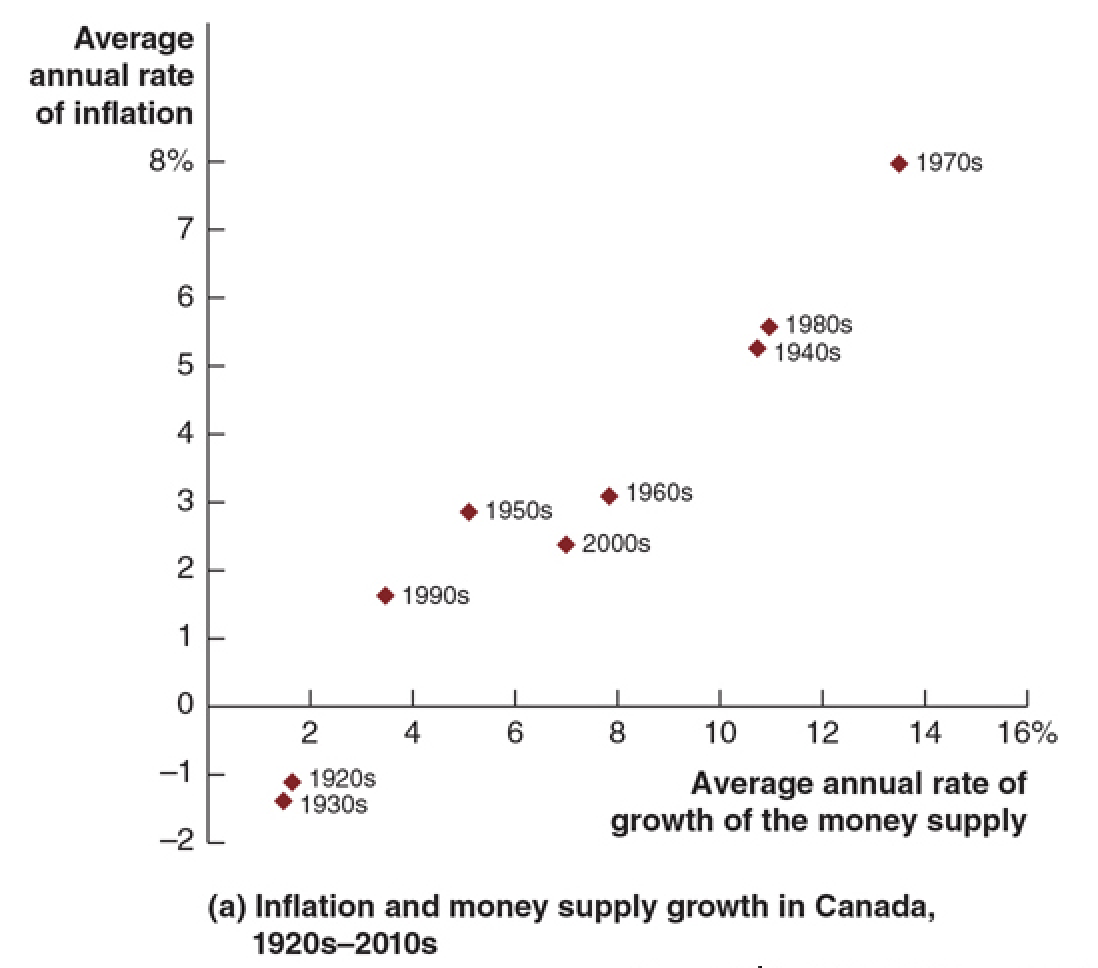
\includegraphics[width=0.5\linewidth]{Fig10-007a}
\end{frame}

\begin{frame}{Figure 10.7 -- Money Growth and Inflation (2 of 2)}
\centering
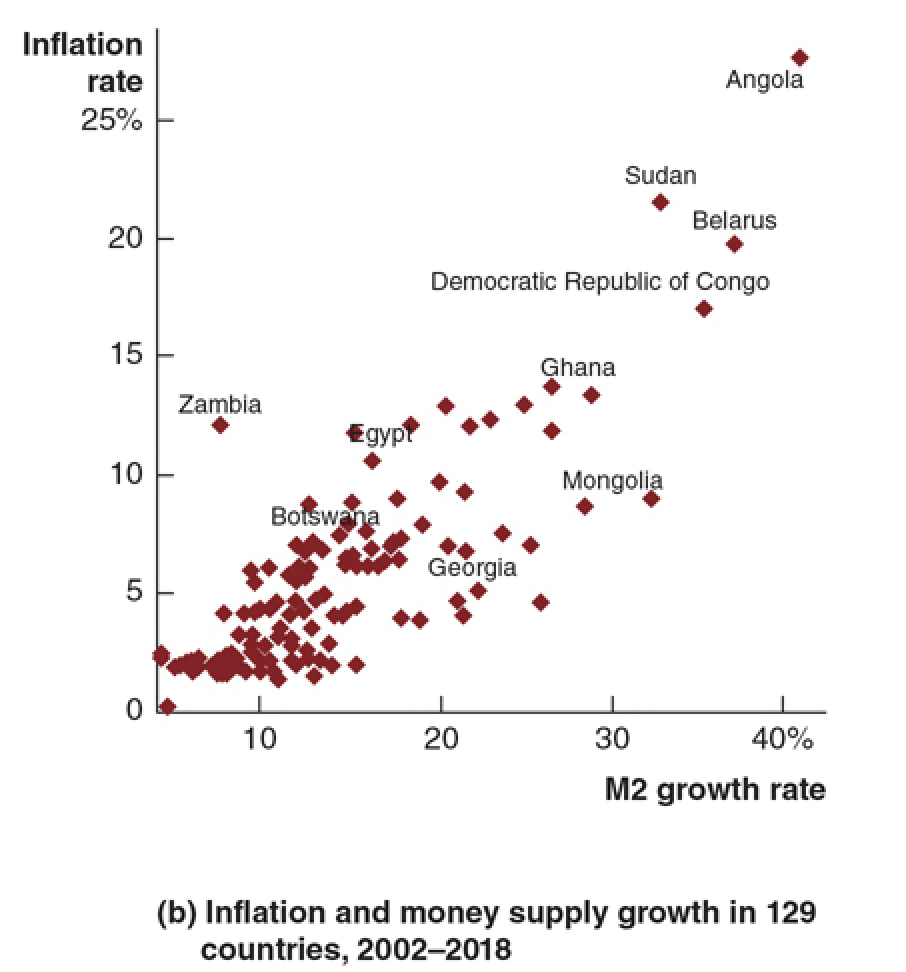
\includegraphics[width=0.5\linewidth]{Fig10-007b}
\end{frame}

\begin{frame}{Money Growth and Inflation: Interpretation}
\transfade
\begin{itemize}[<+->]
  \item Real GDP growth (\(g_{Y}\)) tends to be relatively stable over long periods.
  \item The quantity theory therefore predicts:
  \begin{itemize}[<+->]
    \item a broadly positive relationship between money growth and inflation.
  \end{itemize}
  \item Empirically:
  \begin{itemize}[<+->]
    \item countries with higher average money growth have higher average inflation,
    \item especially when looking at long time spans or very high inflation episodes.
  \end{itemize}
\end{itemize}
\end{frame}

\begin{frame}{High Inflation and Hyperinflation}
\transfade
\begin{itemize}[<+->]
  \item \textbf{Hyperinflation:}
  \begin{itemize}[<+->]
    \item extremely high inflation, often defined as \alert{more than 50\% per month}.
  \end{itemize}
  \item Hyperinflation typically occurs when:
  \begin{itemize}[<+->]
    \item central banks increase the money supply far faster than real GDP,
    \item often because governments are financing very large budget deficits by printing money.
  \end{itemize}
  \item Example:
  \begin{itemize}[<+->]
    \item Zimbabwe experienced hyperinflation so severe that people stopped using the national currency.
  \end{itemize}
  \item Hyperinflation is usually associated with:
  \begin{itemize}[<+->]
    \item very poor economic performance,
    \item deep recessions or even economic collapse.
  \end{itemize}
\end{itemize}
\end{frame}

\begin{frame}{Quantity Theory: Main Takeaway}
\transfade
\begin{itemize}[<+->]
  \item The quantity theory of money is a \textbf{long-run} theory.
  \item It emphasizes that:
  \begin{itemize}[<+->]
    \item \alert{persistent inflation} is ultimately a monetary phenomenon.
    \item In the long run, sustained high inflation requires:
    \[
      g_{M} \gg g_{Y}.
    \]
  \end{itemize}
  \item Central banks that keep money growth close to real GDP growth:
  \begin{itemize}[<+->]
    \item can maintain low and stable inflation over time.
  \end{itemize}
\end{itemize}
\end{frame}

% ============================================================
\section*{Chapter Summary}
% ============================================================

\begin{frame}{Summary}
\transfade
\begin{itemize}[<+->]
  \item Money is any asset widely accepted in exchange for goods, services, or debt payments.
  \item Money performs four key functions:
  \begin{itemize}[<+->]
    \item medium of exchange,
    \item unit of account,
    \item store of value,
    \item standard of deferred payment.
  \end{itemize}
  \item Canada’s money supply has several measures; we emphasize M1+ for its role as a medium of exchange.
  \item Banks create money by accepting deposits and making loans, subject to their desired reserve ratio.
  \item The simple deposit multiplier equals \(1 / r_{d}\), but the real-world multiplier is smaller.
  \item The quantity theory of money links long-run inflation to the growth rate of the money supply relative to real GDP.
\end{itemize}
\end{frame}

\begin{frame}
\centering
\Huge \textbf{Thank you!}
\end{frame}

\end{document}
